\documentclass[tikz = true]{standalone}


\usepackage{amsmath}
\usepackage{amsfonts}
\usepackage{amssymb}
\usepackage{graphicx}
\usepackage{tikz}
\usetikzlibrary{positioning, calc}
\usetikzlibrary{intersections}
\usetikzlibrary{decorations.pathreplacing}
\usetikzlibrary{decorations.text}
\usetikzlibrary{arrows,shapes,backgrounds, shadows,fadings}

\usepackage{fontspec}
\setmainfont{Equity Text A}[SmallCapsFont={Equity Caps A}]

\begin{document}
	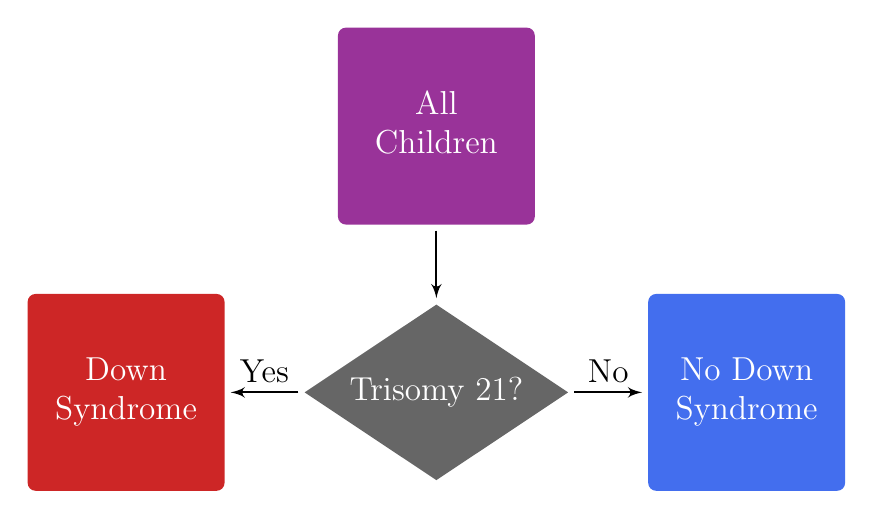
\begin{tikzpicture}
    [node distance=1cm and 1cm,
    post/.style={->,draw,shorten >=2pt,shorten <=2pt,>=latex', thick, font=\large}, 
    ob/.style={rectangle,inner sep=1mm, minimum width=2.5cm, minimum height=2.5cm, rounded corners=1mm,font=\large, text = white}]
    \definecolor{firebrick2}{RGB}{205,38,38};
    \definecolor{royalblue2}{RGB}{67,110,238};
    \node [ob,fill=violet!80] (All) at (0,0) {\begin{tabular}{c} All\\Children\end{tabular}};
    \node (Trisomy) [shape=diamond, below= of All,fill=black!60,shape aspect=1.5, text = white, font = \large] {Trisomy 21?};
    \node [ob,fill=firebrick2,left=of Trisomy] (Down) {\begin{tabular}{c} Down\\Syndrome\end{tabular}};
    \node [ob,fill=royalblue2, right=of Trisomy] (NoDown) {\begin{tabular}{c} No Down\\Syndrome\end{tabular}}; 
    \draw[post] (All) to (Trisomy);
    \draw[post] (Trisomy) -- (Down) node [midway,above] {Yes};
    \draw[post] (Trisomy) -- (NoDown) node [midway,above] {No};
\end{tikzpicture}
\end{document}